
\begin{frame} \frametitle{Motivation}
\begin{itemize}
\item {\bf Primary Goal: } Want to judge the strength \& limitations of
      a game-play heuristic
\item Domain experts model `winning` strategies
\item Want to then visualize the probabilistic effects of changing the
      values of parameters in the state space
\item A {\bf probabilistic map} of the state space where the domain expert
      specifies interesting variables to plot distributions over
\end{itemize}
\end{frame}

\begin{frame} \frametitle{MCMC Sampling Methods}
\begin{itemize}
\item Rejection Sampling - known model for joint distribution
\item Random Walk
  \begin{itemize}
  \item Metropolis-Hastings - known model for joint distribution
  \item Gibbs Sampling - for hard-to-sample joint distribution
  \end{itemize}
\end{itemize}
\begin{columns}
  \column{.45\linewidth}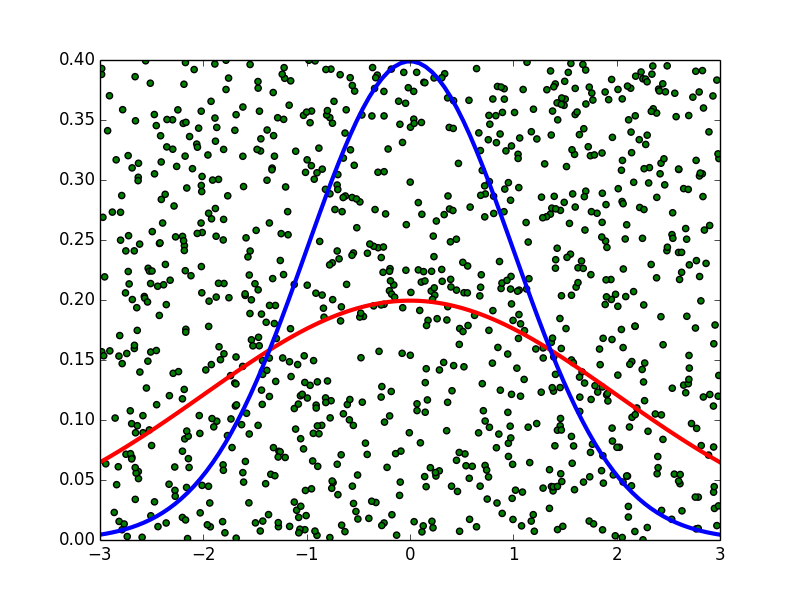
\includegraphics[width=\columnwidth]{rejection_sampling.png}
  \column{.45\linewidth}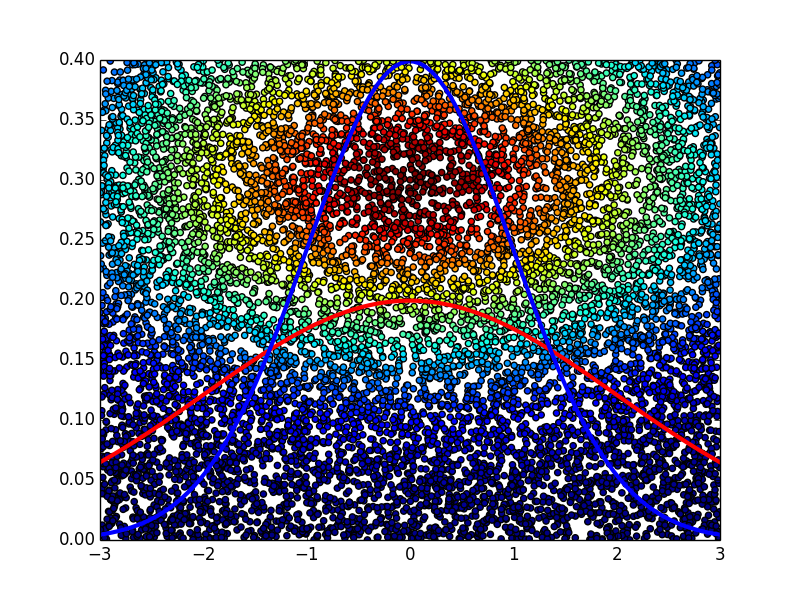
\includegraphics[width=\columnwidth]{metropolis_hastings.png}
\end{columns}
\end{frame}

\begin{frame} \frametitle{Probabilistic Languages}
\begin{itemize}
\item {\bf Hakaru:} an EDSL in Haskell
  \begin{itemize}
  \item Powerful host language support (fully embedded)
  \item Somewhat lacking in domain-specific features (limited API)
  \end{itemize}
\item {\bf BLOG:} a Java-based DSL
  \begin{itemize}
  \item Poweful model of computation (many-worlds modeling)
  \item Lacking in domain-specific tool support and language features
  \end{itemize}
\item Our discussion could be extended to Church, Figaro,
      Fun, others languages discussed in class...
\item Focus on Hakaru for this presentation
% Talk about why other languages were not chosen
\end{itemize}
\end{frame}

\begin{frame}[fragile=singleslide] \frametitle{Sampling - Hakaru}
\begin{minted}
[ frame=lines
, framesep=2mm
, fontsize=\tiny
, linenos
] {haskell}
  test :: IS.Measure Double
  test  = IS.unconditioned (normal (-3) 1)
  test2 = IS.unconditioned (uniform 1 5)

  do
    t  <- IS.sample test []
    let s  = take 1000 $ map fst t
    t2 <- IS.sample test2 []
    let s2 = take 1000 $ map fst t2
    return (makeHistogram 30 (V.fromList (s ++ s2)) "Histogram")
\end{minted}

\begin{columns}
  % FIRST COLUMN
  \column{.6\linewidth} 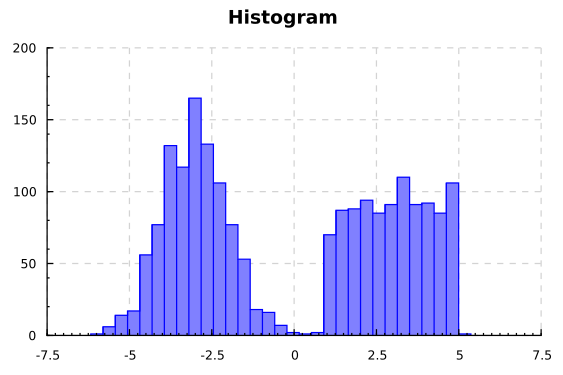
\includegraphics[width=\columnwidth]{hakaru_histogram.png}
  % SECOND COLUMN
  \column{.48\linewidth}
    \begin{itemize}
    \item Can arbitrarily compose Hakaru with Haskell code - single syntax
    \item Conditioned sampling on recursive models?
    \end{itemize}
\end{columns}
\footnotetext[1]{
  {\tiny Example taken from
   \href{http://indiana.edu/~ppaml/HakaruTutorial.html}
        {http://indiana.edu/~ppaml/HakaruTutorial.html}
  }
}
\end{frame}

\begin{frame} \frametitle{Case Study: Deckbuilding Games}
\begin{itemize}
% TODO: reference to Vaccarino from here:
\item We chose \emph{Dominion}\footnotemark to model in a probabilistic language
\item {\bf The Process:}
  \begin{itemize}
  % Actual game engine capable of playing a game - probabilities arise
  % from the underlying mechanics of how and when decks are shuffled,
  % and probabilities *can* arise from what cards a player decides to
  % buy or play during their turn.
  \item Write sampling model based on game mechanics \emph{Dominion}
  \item Determine interesting state variables to condition on
  \item Run Hakaru MCMC
  \item Plot resulting joint distributions for domain expert to explore
  \end{itemize}
\end{itemize}
\footnotetext[1]{{\tiny by \emph{D. X. Vaccarino}}}
\end{frame}

\begin{frame}[fragile=singleslide] \frametitle{Case Study: Dominion Mechanics}
\begin{center}
\begin{Verbatim}[fontsize=\tiny]
λ> runGreedy (0.5, 0.5)
Player1:
    name   = "Greedy1"
    hand   = [ESTATE, GOLD, PROVINCE, PROVINCE, SILVER]
    inPlay = []
    deck   = [SILVER,   PROVINCE, COPPER, SILVER,  COPPER
             ,ESTATE,   COPPER,   COPPER, VILLAGE, VILLAGE
             ,PROVINCE, ESTATE,   SILVER, COPPER]
    dscrd  = [SILVER, SILVER, SILVER, COPPER, COPPER, PROVINCE]
    buys=1, actions=1, money=0

Player2:
    name   = "Greedy2"
    hand   = [COPPER, COPPER, COPPER, COPPER, VILLAGE]
    inPlay = []
    deck   = [SILVER,   SILVER, GOLD, COPPER, COPPER,   ESTATE
             ,GOLD,     ESTATE, GOLD, ESTATE, PROVINCE, VILLAGE
             ,PROVINCE, GOLD]
    dscrd  = [SILVER, COPPER, SILVER, SILVER, SILVER, PROVINCE]
    buys=1, actions=1, money=0

Trash: []
Supply: [(COPPER,60),  (CELLAR,10),  (MOAT,10),       (ESTATE,8)
        ,(SILVER,27),  (VILLAGE,6),  (WOODCUTTER,10), (WORKSHOP,10)
        ,(MILITIA,10), (REMODEL,10), (SMITHY,10),     (MARKET,10)
        ,(MINE,10),    (DUCHY,8),    (GOLD,25),       (PROVINCE,0)]
Turn #: 30
\end{Verbatim}
\end{center}
\end{frame}

\begin{frame}[fragile=singleslide] \frametitle{Case Study: Choice of Parameters}
\begin{itemize}
\item Initially focus on binary choices in card-buying-heuristic
  \begin{itemize}
  \item If we have $3$ treasure on a turn...
    \begin{itemize}
    \item Buy \verb|VILLAGE| with probability $p0$
    \item Buy \verb|CHANCELLOR| with probability $p1 = 1 - p0$
    \end{itemize}
  \item Condition on number of turns in a game
  \item What does the distribution $P(p0 | turns = t)$ for some $t$ look like?
  \end{itemize}
% TODO: put in FUTURE section - non-binary choices
\end{itemize}
\begin{columns}
  \column{.48\linewidth} \begin{flushright} 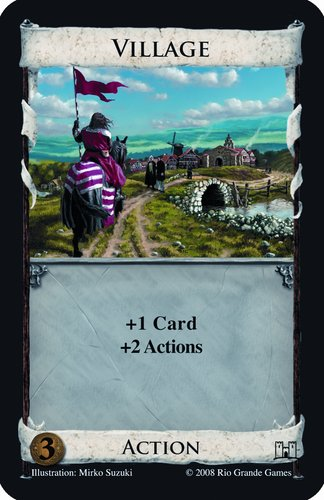
\includegraphics[width=.45\columnwidth]{village.jpg}    \end{flushright}
  \column{.48\linewidth} \begin{flushleft}  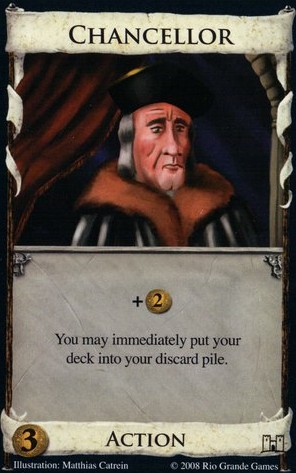
\includegraphics[width=.45\columnwidth]{chancellor.jpg} \end{flushleft}
\end{columns}
\footnotetext[1]{\tiny card content by D. X. Vaccarino}
\end{frame}

\begin{frame} \frametitle{Case Study: Greedy vs Greedy Dominion}
% TODO: itemize
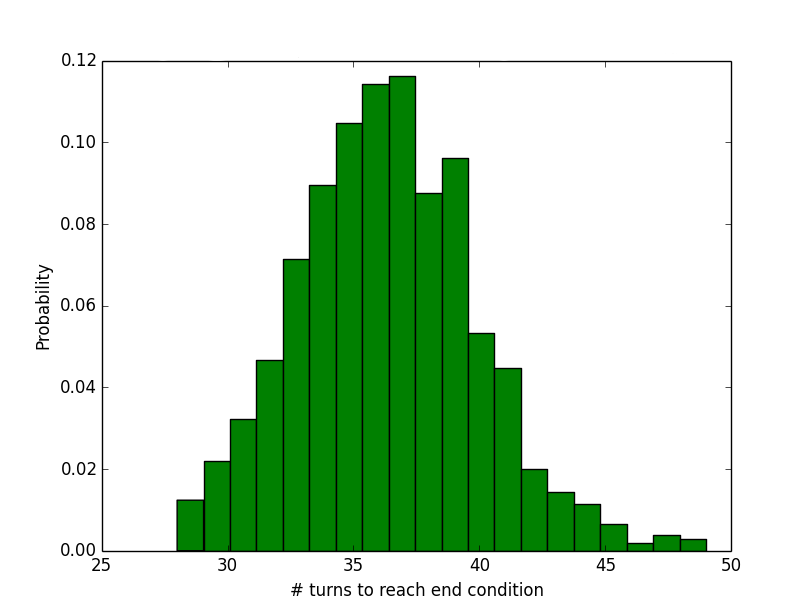
\includegraphics[width=.95\columnwidth]{village-chancellor-turn-dist.png}
\end{frame}

\foreach \n in {40,...,25}{
\begin{frame} \frametitle{Case Study: Rejection Sampling} \includegraphics[width=.95\columnwidth]{../data/village-chancellor-\n turns.png} \end{frame}
}

\begin{frame} \frametitle{Case Study: Future}

\end{frame}

